% 2010 年江苏卷第 16 题：四棱锥 P-ABCD。
% 来源 PDF：普通高考/2010/2010江苏.pdf，SHA-256 e701df878d51a700720549274fe7969bd54342f0f58acb051c516fc502b58af7。
% 原页：第 1 页（A3 三栏）第 3 栏下部，书页码 605。
% 重绘依据：D(0,0,0)、C(1,0,0)、B(1,1,0)、A(-1,1,0)、P(0,0,1)；
%   PD⊥底面，PD=DC=BC=1，AB=2，∠BCD=90°。PD 为高，画虚线。
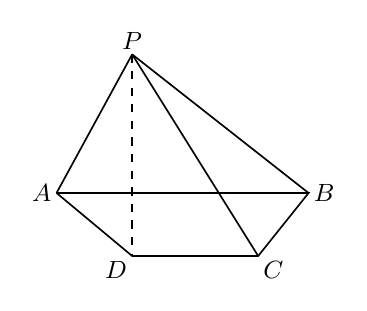
\begin{tikzpicture}[semithick, scale=1.6, every node/.style={inner sep=1.6pt, font=\small}]
  \coordinate (D) at (0,0);
  \coordinate (C) at (1,0);
  \coordinate (B) at (1.4,0.5);
  \coordinate (A) at (-0.6,0.5);
  \coordinate (P) at (0,1.6);

  \draw (A) -- (B) -- (C) -- (D) -- (A);
  \draw (P) -- (A);
  \draw (P) -- (B);
  \draw (P) -- (C);
  \draw[dashed] (P) -- (D);

  \node[below left] at (D) {$D$};
  \node[below right] at (C) {$C$};
  \node[right] at (B) {$B$};
  \node[left] at (A) {$A$};
  \node[above] at (P) {$P$};
\end{tikzpicture}
